% ============================================================
% CAPÍTULO 1 — A ARTE DE COMBINAR INFORMAÇÕES
% ============================================================

\chapter{A arte de combinar informações}

\begin{center}
\textit{Entre o que o modelo prevê e o que o instrumento observa, buscamos a melhor estimativa possível.}
\end{center}

\section*{Resumo}
Este capítulo apresenta a essência da \textbf{assimilação de dados} (AD): a arte e a ciência de combinar, de forma estatisticamente ótima, diferentes fontes de informação --- o modelo numérico e as observações --- para obter a melhor estimativa possível do estado real de um sistema físico, como a atmosfera.  
Partindo de uma visão intuitiva (interpolação ponderada) e evoluindo para a formulação estatística, introduz-se o conceito central de \textit{peso baseado em erro} e a transição entre o ``ajuste geométrico'' e a ``estimação probabilística''.

% ============================================================
\section{Entre o modelo e a realidade}
% ============================================================

A atmosfera é um sistema contínuo em espaço e tempo, mas nossas medições são \textbf{pontuais, esparsas e imperfeitas}.  
Em qualquer instante, conhecemos apenas uma fração do estado verdadeiro \( \mathbf{x}_t \).  
De acordo com \citet{Lorenc1986}, o problema da previsão numérica do tempo (PNT) é, essencialmente, um \textit{problema de condições iniciais}: pequenas incertezas no estado inicial podem amplificar-se exponencialmente devido à natureza caótica da atmosfera.  

\medskip
Para reduzir essa incerteza, introduz-se o conceito de \textbf{análise atmosférica} --- uma estimativa do estado tridimensional da atmosfera no instante de início da previsão.  
Essa análise deve incorporar tanto as observações disponíveis quanto o conhecimento prévio proveniente do modelo numérico.

\begin{definicao}
Segundo \citet{Kalnay2003}, \textit{assimilação de dados} é o processo de combinar, de forma coerente com as leis físicas e estatísticas, as \textbf{observações} e a \textbf{previsão de curto prazo do modelo} (ou \textbf{background}) para obter a melhor estimativa possível do estado do sistema}.
\end{definicao}

Em notação moderna, o objetivo da assimilação é estimar o vetor de estado \( \mathbf{x}_a \in \mathbb{R}^n \) (análise) a partir de:
\begin{itemize}
  \item o \textbf{background} \( \mathbf{x}_b \), proveniente de uma previsão de curto prazo, normalmente de 6 ou 12 horas, gerada por um modelo de PNT;
  \item o vetor de \textbf{observações} \( \mathbf{y} \), obtido de instrumentos diversos (estações de superfície, sondagens, satélites, radares, boias etc.);
  \item o \textbf{operador de observação} \( \mathbf{H} \), que transforma as variáveis do modelo para o espaço de observação.
\end{itemize}

Assim, o problema da assimilação é formular matematicamente o melhor compromisso entre a \emph{consistência dinâmica do modelo} e a \emph{fidelidade das observações}.  
Em termos gerais:
\begin{equation}
\boxed{
\text{modelo (background)} + \text{observações} 
\;\longrightarrow\;
\text{análise (estado inicial ótimo)}.
}
\end{equation}

% ------------------------------------------------------------
\subsection*{Histórico e motivação}
% ------------------------------------------------------------

A análise objetiva e, mais amplamente, a assimilação de dados meteorológicos, emergiram da necessidade de combinar observações esparsas e ruidosas com o conhecimento físico representado por modelos numéricos da atmosfera. Essa busca pela melhor representação possível do estado atmosférico sempre esteve no cerne da previsão numérica do tempo (PNT), cuja qualidade depende fortemente das condições iniciais fornecidas ao modelo.

Os primeiros métodos sistemáticos de análise surgiram na década de 1950, quando \cite{Bergthorsson1955} propuseram o primeiro esquema de análise numérica de mapas meteorológicos, utilizando um processo iterativo para ajustar um campo de pressão ao conjunto de observações disponíveis. Pouco depois, \cite{Cressman1959} introduziu um método operacional simples, porém eficaz, de interpolação ponderada, em que as observações contribuem de forma inversamente proporcional à distância ao ponto de grade. O método de Cressman representou um avanço notável por permitir a incorporação automática de novos dados e por sua aplicabilidade operacional em larga escala.

Nos anos 1970, \cite{Barnes1964, Barnes1973} aprimoraram o conceito de ponderação espacial ao introduzir o método que leva seu nome, baseado em filtros recursivos de resposta quase gaussiana. O esquema de Barnes permitiu um controle mais refinado sobre a suavização e a resolução espacial dos campos analisados, servindo de ponte conceitual entre os métodos empíricos iniciais e as formulações estatísticas posteriores.

A formalização estatística dos processos de análise foi consolidada por \cite{Gandin1963}, cuja obra clássica introduziu a \textit{Interpolação Ótima} (OI, do inglês \textit{Optimal Interpolation}). Nesse método, as observações são combinadas com uma estimativa de ``chute inicial'' (ou \textit{background}) de forma a minimizar o erro quadrático médio, ponderado pelas covariâncias de erro de observação e de modelo. Essa formulação marcou a transição dos métodos empíricos para uma base matemática sólida, permitindo a introdução explícita de informações sobre a estrutura de erro e de correlação espacial.

Durante as décadas seguintes, a OI foi amplamente utilizada em centros de previsão e também serviu de fundamento teórico para métodos mais sofisticados de assimilação. O trabalho de \cite{Lorenc1986} foi crucial ao estabelecer a equivalência formal entre a OI e o método variacional de três dimensões (3D-Var), no qual o problema é resolvido como a minimização de uma função de custo quadrática. Essa equivalência abriu caminho para o desenvolvimento dos métodos variacionais de quatro dimensões (4D-Var), que incorporam a evolução temporal das variáveis de estado por meio do modelo de previsão.

Com a evolução da capacidade computacional e o aumento da disponibilidade de observações (particularmente de satélite), surgiram os métodos baseados em \textit{Ensemble}, como o Filtro de Kalman de Conjunto (EnKF; \cite{Evensen2009}) e seus derivados localizados (LETKF; \cite{Hunt2007}). Esses métodos utilizam múltiplas simulações do modelo para estimar estatísticas de erro de forma adaptativa, permitindo uma representação mais realista da incerteza do sistema e de sua evolução temporal.

A partir dos anos 2000, a pesquisa em assimilação de dados passou a explorar estratégias híbridas que combinam as vantagens dos métodos variacionais e de conjunto. Revisões abrangentes como as de \cite{Bannister2017} e \cite{Carrassi2018} destacam que os métodos híbridos, ao mesclar covariâncias estáticas (variacionais) e dinâmicas (ensemble), representam o estado da arte atual na assimilação de dados geofísicos.

Do ponto de vista histórico, pode-se perceber uma clara progressão: dos métodos empíricos e determinísticos (Cressman, Barnes) para formulações estatísticas e probabilísticas (Gandin, Lorenc, Evensen). Do ponto de vista motivacional, a assimilação de dados evolui continuamente em resposta à crescente complexidade dos sistemas observacionais e à necessidade de estimar, com precisão e consistência física, o estado do sistema atmosférico. Essa evolução reflete o esforço coletivo da comunidade científica em integrar teoria, observação e modelagem numérica em um arcabouço unificado e matematicamente consistente.


\begin{comentario}
O avanço da assimilação de dados ao longo das últimas décadas foi impulsionado por três eixos complementares:
\begin{enumerate}
  \item \textbf{Expansão e diversificação das observações:} a partir da década de 1970, o surgimento de satélites meteorológicos e de novos sensores remotos (radiômetros, sondadores, radar Doppler) aumentou drasticamente a quantidade e a cobertura espacial das medições atmosféricas. Essa revolução observacional exigiu métodos capazes de integrar milhões de dados heterogêneos em tempo quase real.
  \item \textbf{Evolução do poder computacional:} o crescimento exponencial da capacidade de processamento tornou viável a solução iterativa de sistemas lineares e não lineares de alta dimensão, permitindo a transição de métodos empíricos (Cressman, Barnes) para esquemas estatísticos e variacionais (Gandin, Lorenc, Kalnay).
  \item \textbf{Aperfeiçoamento metodológico:} desde a formalização da Interpolação Ótima nos anos 1960 até os métodos híbridos variacional-ensemble atuais, a assimilação de dados evoluiu para representar explicitamente a incerteza e a dinâmica não linear do sistema atmosférico.
\end{enumerate}

Atualmente, centros operacionais globais como o ECMWF, NCEP e JMA realizam análises completas do estado da atmosfera a cada 6 horas, assimilando \textit{centenas de tipos distintos de observações} — desde dados convencionais de superfície até perfis de radiância de satélite — em grades de até dezenas de milhões de variáveis de estado. Essa integração contínua de observações e modelos constitui um dos maiores empreendimentos científicos e computacionais da atualidade.
\end{comentario}

% ------------------------------------------------------------
\subsection*{Interpretação física}
% ------------------------------------------------------------

A assimilação de dados pode ser entendida como um processo de \textbf{fusão de informação física e estatística}, no qual se busca combinar, de forma consistente, o que se sabe pela modelagem e o que se observa da realidade.

\begin{itemize}
  \item O \textbf{modelo numérico} fornece coerência espaço-temporal e obediência às leis fundamentais da dinâmica atmosférica (conservação de massa, momento e energia). Contudo, ele é apenas uma representação aproximada da natureza, sujeita a erros de parametrização e incertezas de condições iniciais e de contorno;
  \item As \textbf{observações} trazem informação direta sobre o estado real da atmosfera, mas são limitadas em cobertura, densidade e precisão, além de conter ruído instrumental e de representatividade espacial.
\end{itemize}

A combinação desses dois mundos segue o princípio da \textbf{melhor estimativa estatística} --- formalizado por \citet{Kalman1960} e generalizado para sistemas atmosféricos por \citet{Lorenc1986}.  
Conceitualmente, desejamos encontrar o estado analisado \( \mathbf{x}_a \) que minimize o erro quadrático médio esperado em relação ao estado verdadeiro \( \mathbf{x}_t \):

\begin{equation}
E\big[(\mathbf{x}_a - \mathbf{x}_t)(\mathbf{x}_a - \mathbf{x}_t)^{\mathrm{T}}\big] 
\;\; \text{mínimo.}
\end{equation}


Esse princípio traduz-se, em sua forma mais simples, na conhecida equação de análise:

\begin{equation}
\mathbf{x}_a = \mathbf{x}_b + \mathbf{K}\big(\mathbf{y} - \mathbf{H}\mathbf{x}_b\big),
\end{equation}

onde:
\begin{itemize}
   \item \( \mathbf{x}_b \) é o \gls{chute inicial} (\textit{first guess} ou ainda \textit{background}), geralmente proveniente da integração anterior do modelo;     
  \item \( \mathbf{y} \) representa o vetor de observações;
  \item \( \mathbf{H} \) é o operador de observação que projeta o espaço do modelo no espaço das observações;
  \item \( \mathbf{K} \) é a \textbf{matriz de ganho}, que pondera a influência relativa do modelo e das observações.
\end{itemize}

%\begin{tcolorbox}[colback=gray!10!white,title={Definição: Chute inicial (\textit{first guess} ou \textit{background})}]
\begin{definicao}
O \textbf{chute inicial} é a previsão de curto prazo utilizada como ponto de partida no processo de assimilação de dados.  
Ele representa a melhor estimativa disponível do estado atmosférico antes da incorporação das observações mais recentes.  
Em sistemas operacionais, o chute inicial é tipicamente obtido pela integração do modelo de previsão a partir da análise anterior.
\end{definicao}
%\end{tcolorbox}


%\begin{tcolorbox}[colback=blue!10!white,title={Nota conceitual: o princípio do BLUE}]
\begin{nota}
A condição de ``melhor estimativa estatística'' em um sistema linear e gaussiano corresponde ao chamado \textit{Best Linear Unbiased Estimator} (BLUE) --- o melhor estimador linear não-viesado.  
Nesse caso, a matriz de ganho de Kalman é dada por:
\[
\mathbf{K} = \mathbf{B}\mathbf{H}^\mathrm{T}(\mathbf{H}\mathbf{B}\mathbf{H}^\mathrm{T} + \mathbf{R})^{-1},
\]
onde \( \mathbf{B} \) e \( \mathbf{R} \) são, respectivamente, as covariâncias dos erros do chute inicial e das observações.  
Essa expressão minimiza a variância do erro de análise e constitui a base matemática da Interpolação Ótima e do Filtro de Kalman --- o núcleo estatístico da assimilação de dados moderna.
\end{nota}
%\end{tcolorbox}

Fisicamente, o processo de assimilação pode ser interpretado como uma \textbf{correção dinâmica}: as observações “ajustam” o modelo em direções onde há informação confiável, enquanto o modelo propaga coerentemente essas correções no espaço e no tempo.  
Essa ponderação é determinada pelas matrizes de covariância de erro:
\begin{itemize}
  \item \( \mathbf{B} \): covariância de erro do \textit{chute inicial}, que expressa a confiança no modelo e define o grau de suavização espacial das análises;
  \item \( \mathbf{R} \): covariância de erro de observação, que quantifica o ruído instrumental e de representatividade.
\end{itemize}

De modo análogo a um filtro passa-baixas em processamento de sinais, a assimilação atua como um \textbf{filtro ótimo} que combina duas fontes de informação com diferentes escalas e níveis de ruído.  
No limite em que as observações são muito precisas (\( \mathbf{R} \to 0 \)), a análise se aproxima dos dados medidos; no limite oposto (\( \mathbf{B} \to 0 \)), confia-se inteiramente no modelo.

Geometricamente, o vetor \( \mathbf{x}_a \) pode ser visto como o ponto de equilíbrio entre duas nuvens de incerteza no espaço de estados — uma associada ao modelo e outra às observações — ponderadas pelas inversas de suas covariâncias.  
Essa visão geométrica é fundamental para compreender as extensões dos métodos variacionais e de \textit{ensemble}, nos quais a assimilação não é apenas uma fusão instantânea, mas um processo contínuo de ajuste no espaço-tempo.

Em métodos como o 4D-Var e o EnKF, essa fusão é realizada dinamicamente: o modelo atua como um “veículo” que transporta a informação das observações ao longo do tempo, garantindo que a coerência física e a estatística caminhem lado a lado.

Em síntese, a assimilação de dados representa a busca pela \textbf{melhor estimativa física e estatisticamente consistente} do estado atmosférico, a partir da combinação otimizada de previsões numéricas e observações reais — o elo essencial entre o mundo modelado e o mundo observado.

% ------------------------------------------------------------
\subsection*{O ciclo de assimilação}
% ------------------------------------------------------------

A assimilação de dados é um processo dinâmico e iterativo, em que observações e previsões de curto prazo são combinadas de forma estatisticamente ótima para estimar o estado mais provável da atmosfera. Esse procedimento é repetido de maneira cíclica, compondo o chamado \textit{ciclo de assimilação} (Figura~\ref{fig:cycle}), que constitui o núcleo operacional de qualquer sistema moderno de previsão numérica.

De forma esquemática, o ciclo segue as seguintes etapas \citep{Kalnay2003}:

\begin{enumerate}
    \item parte-se de um \textbf{campo de background} \( \mathbf{x}_b \), proveniente de uma previsão curta (geralmente de 6 horas), que representa o melhor estado conhecido do sistema antes da incorporação das novas observações;
    \item são coletadas as \textbf{observações} disponíveis dentro de uma janela de tempo centrada no instante de análise (por exemplo, \(\pm 3\) horas em sistemas globais);
    \item aplica-se o \textbf{método de assimilação} (OI, VAR, EnKF etc.), que combina o background e as observações ponderando suas incertezas, resultando na \textbf{análise} \( \mathbf{x}_a \);
    \item a análise é então utilizada como \textbf{condição inicial} para o modelo numérico, que integra o sistema até o próximo tempo de análise, gerando um novo \( \mathbf{x}_b \) e reiniciando o ciclo.
\end{enumerate}

\begin{figure}[h!]
\centering
\begin{tikzpicture}[>=latex,line join=bevel]

  % ===================== PARÂMETROS GERAIS =====================
  \def\N{4}      % número de setas/etapas no anel
  \def\Gap{12}   % gap angular (graus) entre setas

  % Larguras angulares (calculadas para fechar 360° com N setas + N gaps)
  \pgfmathsetmacro{\Span}{(360-\N*\Gap)/\N} % largura de cada seta (graus)
  \pgfmathsetmacro{\Step}{\Span+\Gap}       % passo angular entre centros
  \pgfmathtruncatemacro{\Nm}{\N-1}          % inteiro seguro p/ foreach

  % Raios do anel (controle da “grossura” das setas)
  \def\Rin{3.05}
  \def\Rmid{3.45}
  \def\Rout{3.95}
  \def\Tip{7}    % “ponta” da seta em graus (3–8 costuma ficar bonito)

  % Fundo (anéis de referência e raio das caixas)
  \def\Cin{\Rin-1.05}     % círculo interno do halo
  \def\Cout{\Rout+0.15}   % raio base para posicionar as caixas

  % ================ FUNDO / HALO (opcional) ====================
  \fill[even odd rule,gray!10] circle (\Cout) circle (\Cin); % halo
  \fill[white,opacity=.90] circle (2.05);                    % miolo claro

  % ================ ESTILOS DE COR PARA AS SETAS ===============
  % Use arrow/0,...,arrow/3. Para mais etapas, defina arrow/4, arrow/5, etc.
  \tikzset{
    arrow/0/.style = {fill=teal!30,   draw=teal!70!black,  very thick, line width=1.2pt},
    arrow/1/.style = {fill=green!30,  draw=green!60!black, very thick, line width=1.2pt},
    arrow/2/.style = {fill=orange!40, draw=orange!70!black,very thick, line width=1.2pt},
    arrow/3/.style = {fill=blue!30,   draw=blue!70!black,  very thick, line width=1.2pt},
    % Estilo das caixas externas:
    infobox/.style = {
      draw=black!40, rounded corners=2.2mm, fill=white, drop shadow,
      text width=4.0cm, align=center, inner sep=4pt
    }
  }

  % ===================== DESENHO DAS ETAPAS =====================
  % Lista robusta com 4 campos: índice / ângulo / âncora / texto.
  % OBS: as âncoras devem ser válidas no TikZ: east, west, north, south.
  %      O ângulo (\theta) determina a direção radial da caixa.
  \foreach \i/\theta/\anch/\etapa in {
    0/  25/west/{\textbf{Previsão curta (modelo)}\\Gera $\mathbf{x}_b$ para a janela seguinte},
    1/ 120/south/{\textbf{Coleta \& CQ das observações}\\Janela centrada na análise; filtros e QC},
    2/ 215/east/{\textbf{Análise (assimilação)}\\$\mathbf{x}_a=\mathbf{x}_b+\mathbf{K}\bigl(\mathbf{y}-\mathcal{H}(\mathbf{x}_b)\bigr)$},
    3/ 305/north/{\textbf{Condições iniciais}\\Propaga $\mathbf{x}_a$ para o próximo ciclo}
  }{
    % Centro e limites angulares da seta i
    \pgfmathsetmacro{\center}{\i*\Step}
    \pgfmathsetmacro{\astart}{\center-0.5*\Span}
    \pgfmathsetmacro{\aend}{\center+0.5*\Span}

    % Seta (texto interno curto: “etapa i”; pode trocar por {} se não quiser texto)
    \arcarrow{\Rin}{\Rmid}{\Rout}{\astart}{\aend}{\Tip}{arrow/\i}{etapa \i}

    % Caixa da etapa i (posição polar: ângulo \theta, raio \Cout)
    %  - anchor=\anch prende a caixa pelo lado indicado (east/west/north/south)
    \node[infobox,anchor=\anch] at (\center:\Cout) {\etapa};
  }

  % ======================= TÍTULO CENTRAL =======================
  \node[align=center, text=black!75]
   {\bfseries Ciclo de \\ \bfseries Assimilação de Dados \\
    Integração contínua\\ modelo e observações\\
    (\textit{novo ciclo})};

\end{tikzpicture}


\caption{Esquema conceitual de um ciclo de assimilação de dados atmosféricos. Cada ciclo integra previsões curtas e novas observações para atualizar o estado do sistema.}
\label{fig:cycle}
\end{figure}

Nos sistemas operacionais modernos, esse procedimento é repetido em intervalos regulares — geralmente a cada 6~horas (00, 06, 12 e 18~UTC) — de modo que o modelo numérico e o sistema observacional permaneçam sincronizados.  
As observações coletadas dentro da janela de tempo — provenientes de sondagens, satélites, aeronaves, boias, estações de superfície, entre outras — são temporalmente ajustadas para representar o mesmo instante de validade do \textit{background}, garantindo consistência temporal na análise.  
Assim, a análise combina a informação mais recente do modelo com as observações disponíveis, preservando a coerência dinâmica e física do sistema atmosférico.

Fisicamente, o ciclo de assimilação pode ser interpretado como um \textbf{processo de realimentação}: o modelo fornece uma estimativa coerente e contínua da atmosfera (o \textit{background}), enquanto as observações corrigem os desvios acumulados na previsão anterior.  
Esse mecanismo iterativo assegura que o modelo se mantenha próximo da realidade observada, ao mesmo tempo em que conserva a coerência dinâmica imposta pelas equações de movimento atmosférico.

Com o decorrer dos ciclos, o sistema \textbf{acumula conhecimento estatístico e físico} sobre o estado da atmosfera, reduzindo progressivamente os erros e aumentando a previsibilidade das simulações numéricas.  
Dessa forma, o ciclo de assimilação não constitui apenas um procedimento técnico, mas um \textbf{mecanismo dinâmico de aprendizado}, no qual modelo e observações se complementam mutuamente na busca pela melhor estimativa possível do estado do sistema.

Em síntese, o ciclo de assimilação atua como um \textit{elo de realimentação} entre o modelo e o sistema de observações, garantindo que a previsão de curto prazo permaneça próxima da realidade observada, enquanto mantém a coerência física e dinâmica exigida pelas equações do modelo.

% ------------------------------------------------------------
\subsection*{Síntese conceitual}
% ------------------------------------------------------------

\begin{sintese}
A assimilação de dados:
\begin{itemize}
    \item reconhece explicitamente que tanto o modelo quanto as observações possuem erro;
    \item combina essas duas fontes de informação com base em suas \textbf{covariâncias de erro};
    \item produz uma estimativa estatisticamente ótima do estado atmosférico;
    \item mantém coerência temporal e física através do ciclo modelo--análise.
\end{itemize}
Em outras palavras, ela é o \textbf{elo entre a teoria, a observação e a modelagem numérica} --- um processo que transforma dados brutos em conhecimento preditivo sobre o Sistema Terrestre.
\end{sintese}


% ============================================================
\section{Interpolação como estimativa ponderada}
% ============================================================

Antes de pensar em estatística, é útil lembrar que a ideia de \textbf{combinar informações} já existia implicitamente na \textbf{interpolação clássica}.  
Nela, a estimativa \( \hat{z}(x_0) \) em um ponto \( x_0 \) é uma média ponderada das observações conhecidas \( z(x_i) \):

\begin{equation}
\hat{z}(x_0) = \sum_{i=1}^{N} w_i(x_0)\, z(x_i),
\qquad 
\sum_{i=1}^{N} w_i(x_0) = 1.
\label{eq:interp}
\end{equation}

Os \textbf{pesos} \( w_i(x_0) \) dependem da distância entre o ponto de interesse e as observações.  
Um exemplo clássico é o \textbf{peso gaussiano}:

\begin{equation}
w_i(x_0)
= 
\dfrac{
\exp\!\left[-\dfrac{(x_0 - x_i)^2}{R^2}\right]
}{
\sum_{j=1}^{N} 
\exp\!\left[-\dfrac{(x_0 - x_j)^2}{R^2}\right]
},
\label{eq:gaussian_weight}
\end{equation}
onde \( R \) é o \textbf{raio de influência}.  
Quanto menor a distância \(|x_0 - x_i|\), maior o peso de \(z(x_i)\) na estimativa.

\medskip
\noindent
\textbf{Interpretação física.}  
A interpolação ponderada já é, implicitamente, uma filtragem espacial: as observações mais próximas (ou mais confiáveis) dominam a estimativa.  
Essa ideia inspirou a \textbf{análise objetiva} \citep{Cressman1959,Barnes1964} --- o elo direto com a assimilação moderna.

% ============================================================
\section{Transição para pesos baseados em erro}
% ============================================================

A grande revolução conceitual da assimilação moderna foi substituir o critério geométrico (distância) por um \textbf{critério estatístico (erro)}.  

Denotemos:
\begin{itemize}
    \item \( \mathbf{x}_b \) --- vetor de background (previsão de curto prazo);
    \item \( \mathbf{y} \) --- vetor de observações;
    \item \( \mathbf{H} \) --- operador que mapeia o estado do modelo para o espaço de observação;
    \item \( \mathbf{K} \) --- matriz de ganho (ou de ponderação ótima).
\end{itemize}

A análise é dada por:
\begin{equation}
\boxed{
\mathbf{x}_a = \mathbf{x}_b + \mathbf{K}\,(\mathbf{y} - \mathbf{H}\mathbf{x}_b)
}
\label{eq:analysis}
\end{equation}
em que o termo \(\mathbf{d} = \mathbf{y} - \mathbf{H}\mathbf{x}_b\) é a \textbf{inovação} (diferença observação--background).

A matriz \(\mathbf{K}\) define o peso ótimo de cada informação:
\begin{equation}
\boxed{
\mathbf{K} = \mathbf{B}\,\mathbf{H}^\mathrm{T}\,
(\mathbf{H}\mathbf{B}\mathbf{H}^\mathrm{T} + \mathbf{R})^{-1}},
\label{eq:kalman_gain}
\end{equation}
onde  
\(\mathbf{B}\) é a covariância de erro de background e  
\(\mathbf{R}\) é a covariância de erro de observação.

Essas matrizes determinam quanto se confia no modelo ou nas observações:

\begin{center}
\begin{tabular}{|c|c|}
\hline
Situação & Consequência \\
\hline
\( \mathbf{B} \gg \mathbf{R} \) & observações recebem maior peso \\
\( \mathbf{R} \gg \mathbf{B} \) & o modelo prevalece \\
\( \mathbf{B} \sim \mathbf{R} \) & combinação equilibrada \\
\hline
\end{tabular}
\end{center}

\noindent
\textbf{Interpretação.}  
A AD é uma \textit{interpolação ponderada por incertezas}, ou seja, uma fusão estatisticamente fundamentada entre modelo e dados.

% ============================================================
\section{Exemplo escalar --- o caso BLUE 1D}
% ============================================================

Considere uma variável escalar \(z\) observada (\(z_o\)) e prevista pelo modelo (\(z_b\)).  
Suponha erros não correlacionados, com variâncias \(\sigma_o^2\) e \(\sigma_b^2\).  
A melhor estimativa linear não enviesada (BLUE, \textit{Best Linear Unbiased Estimator}) é:
\begin{equation}
z_a = 
\dfrac{z_b/\sigma_b^2 + z_o/\sigma_o^2}
      {1/\sigma_b^2 + 1/\sigma_o^2}.
\label{eq:blue}
\end{equation}

ou, de modo equivalente,
\begin{equation}
z_a =
w_b\,z_b + w_o\,z_o,
\qquad
w_b = \dfrac{1/\sigma_b^2}{1/\sigma_b^2 + 1/\sigma_o^2},
\quad
w_o = \dfrac{1/\sigma_o^2}{1/\sigma_b^2 + 1/\sigma_o^2}.
\end{equation}

Se o modelo erra mais (\(\sigma_b^2\) grande), \(w_o\) domina; se as observações são mais ruidosas (\(\sigma_o^2\) grande), \(w_b\) domina.  
A Eq.~\eqref{eq:blue} é a forma unidimensional das Eqs.~\eqref{eq:analysis} e~\eqref{eq:kalman_gain}.

% ------------------------------------------------------------
\begin{tcolorbox}[title={Ligação com mínimos quadrados},colback=gray!5!white]
Minimizar o erro médio quadrático entre a análise e o estado verdadeiro \(x_t\) leva exatamente à Eq.~\eqref{eq:kalman_gain}.  
A matriz \(\mathbf{K}\) surge como solução do problema:
\[
\min_{\mathbf{K}} 
E\big[(\mathbf{x}_a - \mathbf{x}_t)(\mathbf{x}_a - \mathbf{x}_t)^\mathrm{T}\big].
\]
Derivando e anulando o gradiente, obtém-se a solução de Kalman.  
Portanto, o ganho de Kalman é o \textbf{operador de mínimos quadrados generalizado}.
\end{tcolorbox}

% ============================================================
\section{Representação visual (pgfplots)}
% ============================================================

\begin{figure}[h!]
\centering
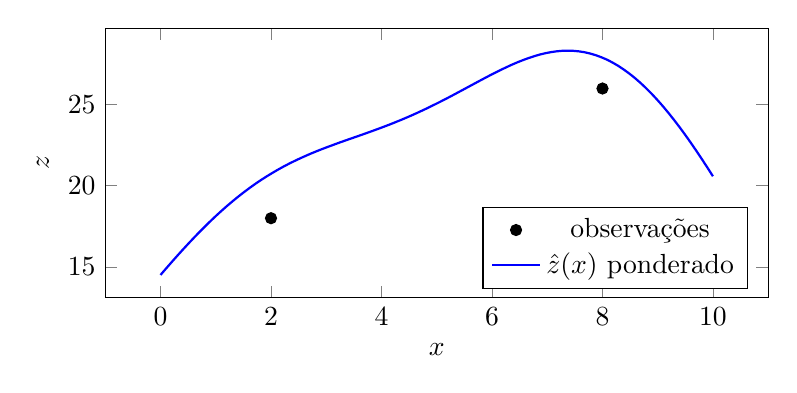
\begin{tikzpicture}
\begin{axis}[xlabel={$x$}, ylabel={$z$}, width=10cm, height=5cm, legend pos=south east]
\addplot[only marks, mark=*] coordinates {(2,18) (8,26)};
\addlegendentry{observações};
\addplot[domain=0:10,samples=100,blue,thick]{18*exp(-(x-2)^2/16)+26*exp(-(x-8)^2/16)};
\addlegendentry{$\hat{z}(x)$ ponderado};
\end{axis}
\end{tikzpicture}
\caption{Interpolação 1D entre duas observações usando pesos gaussianos normalizados (raio efetivo \(R\approx4\)).}
\label{fig:interp1d}
\end{figure}

\begin{figure}[h!]
\centering
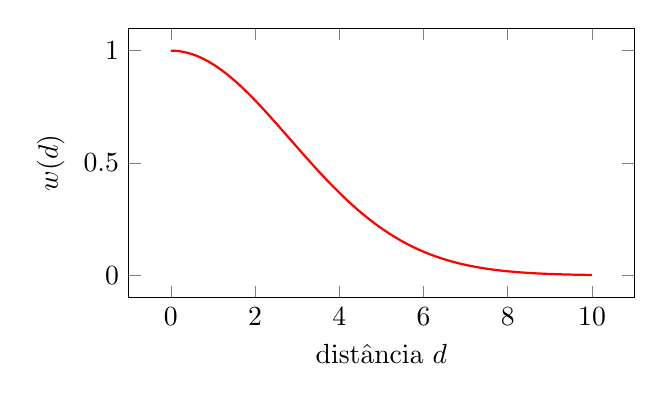
\begin{tikzpicture}
\begin{axis}[xlabel={distância $d$}, ylabel={$w(d)$}, width=8cm, height=5cm]
\addplot[domain=0:10,samples=100,red,thick]{exp(-x^2/16)};
\end{axis}
\end{tikzpicture}
\caption{Função de peso gaussiana típica utilizada em análises espaciais: o peso decai rapidamente com a distância em relação ao raio \(R\).}
\label{fig:gaussian}
\end{figure}

% ============================================================
\section{Interpretação física e probabilística}
% ============================================================

Sob a ótica probabilística,  
\begin{itemize}
    \item o background é uma amostra da distribuição \( \mathcal{N}(\mathbf{x}_t, \mathbf{B}) \);
    \item as observações, uma amostra de \( \mathcal{N}(\mathbf{H}\mathbf{x}_t, \mathbf{R}) \).
\end{itemize}
A análise é a média ponderada dessas duas distribuições --- o ponto em que o \textbf{produto das probabilidades} é máximo.  
Ou seja, o vetor \( \mathbf{x}_a \) é o \textbf{valor de máxima verossimilhança} sob hipóteses gaussianas.

% ============================================================
\section{Síntese}
% ============================================================

A interpolação fornece a intuição básica: estimar valores nos vazios, combinando vizinhança e suavidade.  
A assimilação de dados amplia esse conceito ao incluir \textbf{incertezas estatísticas} e formular a estimativa como uma \textbf{combinação ótima} de modelo e observação.

\begin{equation}
\text{Interpolação} 
\;\Rightarrow\;
\text{Mínimos Quadrados} 
\;\Rightarrow\;
\text{Análise Objetiva} 
\;\Rightarrow\;
\text{Assimilação Estatística (VAR, EnKF, Kalman)}.
\end{equation}

Nos capítulos seguintes, formalizaremos essa transição passo a passo --- do ajuste por mínimos quadrados à formulação completa da assimilação moderna.

% ============================================================
\section*{Referências}
% ============================================================

\begin{thebibliography}{99}
\bibitem[Cressman(1959)]{Cressman1959} Cressman, G. P. (1959). \textit{An operational objective analysis system}. Mon. Wea. Rev., 87, 367--374.
\bibitem[Barnes(1964)]{Barnes1964} Barnes, S. L. (1964). \textit{A technique for maximizing detail in numerical weather map analysis}. J. Appl. Meteor., 3, 396--409.
\bibitem[Kalnay(2003)]{Kalnay2003} Kalnay, E. (2003). \textit{Atmospheric Modeling, Data Assimilation and Predictability}. Cambridge Univ. Press.
\bibitem[Lorenc(1986)]{Lorenc1986} Lorenc, A. C. (1986). \textit{Analysis methods for numerical weather prediction}. Q. J. R. Meteorol. Soc., 112, 1177--1194.
\bibitem[Evensen(2009)]{Evensen2009} Evensen, G. (2009). \textit{Data Assimilation: The Ensemble Kalman Filter}. Springer.
\end{thebibliography}
